% Provenance (never printed): see sources/outline_sources.md (Year 3:
% speciation and saturation indices; carbonate equilibria applied to rocks;
% weathering kinetics; hydrothermal fluids). Brief: sources/book5/BRIEFS.md,
% ch. 15. Curves from figdata/bachelor-3/carbonate_system.py,
% activity_diagram.py, weathering_rates.py. Exercise and problem values in the
% Book 5 scratch calculator calc/ch15.py. The spring below the Varden
% limestone, its analysis and the granite stream are invented.
\chapter{जल--चट्टान अंतर्क्रिया}\label{ch:b3:water-rock-interaction}

चूना-पत्थर की ढलान के तल पर स्थित एक सोता जिस भी टहनी या पत्थर को छूता है,
उस पर सफ़ेद पपड़ी छोड़ता है; ग्रेनाइट से बहने वाली धारा सिलिका, सोडियम
और थोड़ा पोटैशियम ढोती है, और उस पर कोई पपड़ी नहीं बनती। यह अंतर
जल के रासायनिक गुणों में है, और ये गुण उस चट्टान का अभिलेख हैं
जिसे जल ने पार किया: वह कितनी कार्बन डाइऑक्साइड साथ लाया, कितनी देर रुका, कौन से
खनिज उसने घोले और कौन से बनाए। यह अध्याय इस अभिलेख को विलयन रसायन के
उपकरणों से पढ़ता है, जल के विश्लेषण से लेकर खनिज विलयन की दरों तक
और भूपर्पटी में गर्म तरलों के समस्थानिक अनुरेखों तक।

\begin{recall}
सक्रियता, सक्रियता गुणांक, आयनिक सामर्थ्य, स्पीशिएशन, विलेयता
गुणनफल, क्षारीयता, संतृप्ति अवस्था $\Omega$, हेनरी का नियम, दर नियम,
आरहीनियस नियम, संक्रमण अवस्था और $\delta$ मान रसायन की पुस्तकों के
विश्वविद्यालय खंडों में हैं। रासायनिक अपक्षय, सिलिकेटों का जल-अपघटन,
मृत्तिका-खनिज और कैओलिनाइट पुस्तक 3 (स्नातक वर्ष 1) में हैं, उसके
अपक्षय और मृत्तिकाओं वाले अध्याय में; लाइसोक्लाइन और कार्बोनेट प्रतिकरण
गहराई कार्बोनेट, सिलिसियस और वाष्पनिक अवसादों वाले अध्याय में बताई गई है।
जलतापीय तरल पुस्तक 4 (स्नातक वर्ष 2) में है, अयस्क निक्षेपों वाले अध्याय में,
और सिलिकेट-अपक्षय तापस्थापी उस अध्याय में है जो भूवैज्ञानिक काल की जलवायु पर है;
जलतापीय परिसंचरण स्कूली पुस्तकों में है।
\end{recall}

\section{किसी प्राकृतिक जल का विश्लेषण}\label{sec:b3:water-rock-interaction:analysis}

जल विश्लेषण में प्रमुख आयन मिलीग्राम प्रति लीटर में सूचीबद्ध होते हैं: कैल्शियम,
मैग्नीशियम, सोडियम और पोटैशियम; बाइकार्बोनेट, क्लोराइड, सल्फ़ेट और नाइट्रेट;
विलेय सिलिका \ce{SiO2} के रूप में; और स्रोत पर मापे गए pH और तापमान,
क्योंकि नमूना स्रोत से निकलते ही ये दोनों बदल जाते हैं। मोलर द्रव्यमान से भाग देने पर
प्रति लीटर मिलिमोल मिलते हैं, और आवेश से गुणा करने पर
मिलि-तुल्यांक मिलते हैं। तनु जल विद्युत-उदासीन होता है, इसलिए धनायनों का योग
ऋणायनों के योग के बराबर होना चाहिए।

\begin{method}[जल विश्लेषण की जाँच]\label{met:b3:water-rock-interaction:analysis}
\begin{enumerate}
\item प्रत्येक सांद्रता को \unit{mmol/L} और \unit{meq/L} में बदलिए;
\item धनायनों और ऋणायनों का \unit{meq/L} में योग कीजिए;
\item आवेश-संतुलन त्रुटि $100\,(\sum\text{धन} -
  \sum\text{ऋण})/(\sum\text{धन} + \sum\text{ऋण})$, प्रतिशत में परिकलित कीजिए;
\item विश्लेषण स्वीकार कीजिए, यदि त्रुटि 1 या \qty{2}{\percent} के भीतर हो,
  250 से \qty{1000}{mg/L} तक के जल के लिए, अधिक तनु जल के लिए थोड़ी अधिक;
  अन्यथा किसी छूटे आयन या विश्लेषणात्मक त्रुटि को खोजिए।
\end{enumerate}
\end{method}
% ledger: hem85:charge-balance

किसी आयन की सक्रियता उसकी मोललता को उसके सक्रियता गुणांक
$\gamma$ से गुणा करने पर मिलती है। प्राकृतिक जल में $\gamma$ आयनिक सामर्थ्य $I =
\tfrac12\sum m_i z_i^2$ से परिकलित होता है, विस्तारित डेबाई--ह्यूकेल समीकरण के साथ
\[
-\log\gamma_i = \frac{A z_i^2\sqrt I}{1 + B a_i\sqrt I},
\]
\qty{25}{\celsius} पर पानी के लिए $A = 0.5085$ और $B = 0.3281$ हैं, और आयन का
आकार $a_i$ ऐंगस्ट्रॉम में: \ce{H+} के लिए 9, \ce{Mg^2+} के लिए 8,
\ce{Ca^2+} के लिए 6, \ce{CO3^2-} के लिए 5, \ce{Na+}, \ce{HCO3-} और \ce{SO4^2-} के लिए 4,
\ce{K+}, \ce{Cl-}, \ce{OH-} और \ce{NO3-} के लिए 3। यह समीकरण
लगभग \qty{0.1}{mol/L} तक की एक-संयोजी लवण सांद्रता के लिए ठीक है, जो नदियों और अधिकांश
भूजल पर लागू होता है, पर समुद्री जल या ब्राइन पर नहीं। तापमान $A$ का मान केवल
\qty{0}{\celsius} पर 0.4883 से \qty{60}{\celsius} पर 0.5425 तक बदलता है, इसलिए
\qty{25}{\celsius} के मान ठंडे जल पर भी लागू होते हैं।
% ledger: hem85:debye-huckel

जल का अकार्बनिक कार्बन विलेय कार्बन डाइऑक्साइड
(\ce{CO2} लिखा जाता है, जो \ce{CO2} और \ce{H2CO3} का योग है), बाइकार्बोनेट और
कार्बोनेट में बँटा होता है, जो निम्न संबंधों से जुड़े हैं:
\[
K_1 = \frac{a_{\ce{HCO3-}}\,a_{\ce{H+}}}{a_{\ce{CO2}}}, \qquad
K_2 = \frac{a_{\ce{CO3^2-}}\,a_{\ce{H+}}}{a_{\ce{HCO3-}}}, \qquad
K_H = \frac{a_{\ce{CO2}}}{P_{\ce{CO2}}},
\]
इनके मान $\log K_1 = -6.35$, $\log K_2 = -10.33$ और $\log K_H = -1.47$ के
\qty{25}{\celsius} पर बराबर हैं, और \qty{10}{\celsius} पर $-6.46$, $-10.49$ और $-1.27$
($P$ वायुमंडल में)। pH 6.4 और 10.3 के बीच बाइकार्बोनेट प्रधान होता है, और
अधिकांश प्राकृतिक जल में क्षारीयता लगभग पूरी तरह बाइकार्बोनेट होती है। मापा गया pH
और बाइकार्बोनेट से अन्य दो स्पीशीज़ और वह कार्बन डाइऑक्साइड का आंशिक दाब
निकलता है जिसके साथ जल साम्य में होगा।
% ledger: phreeqc:carbonate

\section{संतृप्ति}\label{sec:b3:water-rock-interaction:saturation}

\begin{definition}[संतृप्ति सूचकांक]\label{def:b3:water-rock-interaction:si}
जल में \emph{संतृप्ति सूचकांक}\index{संतृप्ति सूचकांक}
$\mathrm{SI} = \log(\mathrm{IAP}/K)$ है, जहाँ IAP
जल का आयन सक्रियता गुणनफल है, जिसे खनिज के विलेयता
गुणनफल $K$ के समान लिखा जाता है: $\mathrm{SI} = \log\Omega$।
\end{definition}

$\mathrm{SI} < 0$ वाला जल खनिज को घोल सकता है, और $\mathrm{SI} > 0$ वाला
जल उसे अवक्षेपित कर सकता है, और $\mathrm{SI} = 0$ साम्य की अवस्था है।
चूँकि विलयन अभिक्रिया की मुक्त ऊर्जा $\Delta_r G = RT\ln\Omega
= 2.303\,RT\,\mathrm{SI}$ है, अतः \omterm{def:b3:water-rock-interaction:si}{संतृप्ति सूचकांक} भी चालक बल का माप है,
$2.303\,RT$ की इकाइयों में, लगभग \qty{5.7}{kJ/mol} के बराबर
\qty{25}{\celsius} पर। कैल्साइट के लिए $\mathrm{IAP} = a_{\ce{Ca^2+}}
a_{\ce{CO3^2-}}$ है और \qty{25}{\celsius} पर $\log K = -8.45$ तथा
\qty{10}{\celsius} पर $-8.35$: कैल्साइट ठंडे जल में अधिक विलेय है। जिप्सम के लिए, $\mathrm{SI} = \log(a_{\ce{Ca^2+}}a_{\ce{SO4^2-}}) + 4.55$;
क्वार्ट्ज़ के लिए, जिसके विलयन से उदासीन \ce{H4SiO4} बनता है, $\mathrm{SI} = \log
a_{\ce{H4SiO4}} + 3.98$ है, और अनिराकार सिलिका के लिए स्थिरांक 2.71
3.98 के स्थान पर। मापे गए सूचकांकों में कम से कम $\pm0.1$ की
अनिश्चितता होती है, और शून्य से $\pm0.3$ के भीतर के जल को साम्य के निकट माना जाता है।
% ledger: phreeqc:carbonate, phreeqc:silicates, hem85:si

\section{चट्टानों में कार्बोनेट साम्य}\label{sec:b3:water-rock-interaction:carbonate}

कार्बन डाइऑक्साइड से युक्त जल में कैल्साइट निम्न अभिक्रिया द्वारा घुलता है:
\[
\ce{CaCO3 + CO2 + H2O <=> Ca^2+ + 2 HCO3-},
\qquad K = \frac{a_{\ce{Ca^2+}}\,a_{\ce{HCO3-}}^2}{P_{\ce{CO2}}}
= \frac{K_{\mathrm{cal}}K_1K_H}{K_2},
\]
\qty{25}{\celsius} पर $\log K = -5.94$ और \qty{10}{\celsius} पर $-5.59$।
कितना घुलता है, यह इस पर निर्भर करता है कि कार्बन डाइऑक्साइड कहाँ से आती है।

\begin{definition}[खुला और बंद कार्बोनेट तंत्र]\label{def:b3:water-rock-interaction:open-closed}
कोई जल कैल्साइट को \emph{खुला कार्बोनेट तंत्र}\index{खुला कार्बोनेट तंत्र} में
घोलता है, जब वह निश्चित
$P_{\ce{CO2}}$ की गैस के संपर्क में रहता है, जो प्रयुक्त कार्बन डाइऑक्साइड की जगह लेती है।
यही काम वह \emph{बंद कार्बोनेट तंत्र}\index{बंद कार्बोनेट तंत्र} में तब करता है, जब वह
पहले कार्बन डाइऑक्साइड से युक्त हुआ और फिर गैस से पृथक किया गया, ताकि
उसके पास जो कार्बन डाइऑक्साइड है, केवल वही उसके उपयोग में आ सकती है।
\end{definition}

\begin{theorem}[कैल्साइट की विलेयता, खुला और बंद]\label{thm:b3:water-rock-interaction:calcite}
कैल्शियम बाइकार्बोनेट प्रकार के जल के लिए, जिसमें $m$ कैल्शियम की मोलता है,
\[
\text{खुला:}\quad m = \left(\frac{K\,P_{\ce{CO2}}}{4\gamma_{\ce{Ca^2+}}
\gamma_{\ce{HCO3-}}^2}\right)^{1/3};
\qquad
\text{बंद:}\quad 4\gamma_{\ce{Ca^2+}}\gamma_{\ce{HCO3-}}^2\,m^3 =
\frac{K_{\mathrm{cal}}K_1}{K_2}\,(C_0 - m),
\]
जहाँ $C_0 = K_H P_{\ce{CO2}}$ वह कार्बन डाइऑक्साइड है जो
तंत्र बंद होने से पहले अवशोषित हुई थी।
\end{theorem}

\begin{proof}
pH 6.5 और 8.5 के बीच कार्बोनेट, \ce{H+} और \ce{OH-} बाइकार्बोनेट की तुलना में
नगण्य होते हैं, इसलिए आवेश-संतुलन $2m = m_{\ce{HCO3-}}$ है। खुला: $K = \gamma
_{\ce{Ca^2+}}m\,\gamma_{\ce{HCO3-}}^2(2m)^2/P_{\ce{CO2}}$, जिससे घनमूल
प्राप्त होता है। बंद: घुले हुए प्रत्येक कैल्शियम के लिए एक \ce{CO2} प्रयुक्त होता है, इसलिए $m_{\ce{CO2}}
= C_0 - m$ और $a_{\ce{Ca^2+}}a_{\ce{HCO3-}}^2/a_{\ce{CO2}} = K/K_H =
K_{\mathrm{cal}}K_1/K_2$ से घन समीकरण प्राप्त होता है।
\end{proof}

खुले तंत्र में कैल्शियम $P_{\ce{CO2}}$ के घनमूल के अनुसार बढ़ता है; बंद तंत्र में
वह $C_0$ द्वारा सीमित रहता है, और अंत में बची
कार्बन डाइऑक्साइड, अतः अंतिम $P_{\ce{CO2}}$, आरंभ की तुलना में बहुत कम होता है।
मिट्टी की हवा में वायुमंडल से 10 से 100 गुना कार्बन डाइऑक्साइड होती है, जो जड़ों
और पादप-पदार्थ के अपघटन से बनती है, तथा भूजल सामान्यतः
$P_{\ce{CO2}}$ का $10^{-2.5}$ और $10^{-1}$ वायुमंडल के बीच मान दिखाते हैं। कैल्साइट और वायु के संपर्क वाला जल
में केवल लगभग \qty{20}{mg/L} कैल्शियम होता है; वह वर्षा जल जो
मिट्टी से होकर चूना-पत्थर तक पहुँचता है और मिट्टी की गैस के लिए अब भी खुला है, वह
चार या पाँच गुना अधिक घोल सकता है। कार्स्ट भूदृश्य इसी मिट्टी की कार्बन डाइऑक्साइड से गढ़ा जाता है।
% ledger: hem85:pco2, phreeqc:carbonate

वापसी का मार्ग गैस-निष्कासन है। चूना-पत्थर से निकलने वाला सोता
मिट्टी और चट्टान का $P_{\ce{CO2}}$, जो वायु के दस से सौ गुना
है, ले जाता है। खुले में यह कार्बन डाइऑक्साइड खोता है, बाइकार्बोनेट
कार्बोनेट में बदल जाता है, pH बढ़ता है, और \omterm{def:b3:water-rock-interaction:si}{संतृप्ति सूचकांक} एक इकाई से अधिक बढ़ जाता है,
जैसा कि नीचे के चित्र के पैनल (ख) में इस अध्याय की
सप्ताहांत समस्या वाले सोते के लिए दिखाया गया है।
कैल्साइट धारा की तली पर और काई तथा टहनियों पर अवक्षेपित होता है: ठंडे सोतों से
टफ़ा, और गर्म सोतों से ट्रैवर्टीन। जो सोते चट्टान से होकर
तेज़ी से, दिनों या हफ़्तों में, नलिकाओं द्वारा गुज़रते हैं, वे सामान्यतः
असंतृप्त अवस्था में सतह पर पहुँचते हैं; जो सोते महीनों तक धीरे-धीरे उसमें से रिसते हैं,
वे संतृप्ति के निकट निकलते हैं।
% ledger: hem85:pco2, usgsyvo:travertine

\begin{omfigure}
\begin{tikzpicture}
\begin{groupplot}[group style={group size=2 by 1, horizontal sep=1.6cm},
  omrecord, width=0.47\linewidth, height=0.42\linewidth, title style={font=\small},
  tick label style={font=\scriptsize}, label style={font=\small},
  legend style={font=\scriptsize, legend cell align=left}]
\nextgroupplot[title={(क) कैल्साइट विलेयता},
  xlabel={$\log P_{\ce{CO2}}$ (वायुमंडल)}, ylabel={घुला कैल्शियम (\unit{mmol/L})},
  xmin=-3.5, xmax=-1, ymin=0, ymax=5.5, clip=false,
  xtick={-3.5,-3,-2.5,-2,-1.5,-1}, xticklabels={$-3.5$,$-3$,$-2.5$,$-2$,$-1.5$,$-1$},
  legend style={at={(0.14,0.97)}, anchor=north west}]
\addplot[draw=none, fill=black!6, forget plot] coordinates {(-2.5,0) (-2.5,5.5) (-1,5.5) (-1,0)} -- cycle;
% computed in figdata/bachelor-3/carbonate_system.py
\addplot[omDef, thick] table[x=logp, y=ca_open10] {figdata/out/bachelor-3-carbonate_system-solubility.dat};
\addlegendentry{खुला, \qty{10}{\celsius}}
\addplot[red!70!black, thick] table[x=logp, y=ca_open25] {figdata/out/bachelor-3-carbonate_system-solubility.dat};
\addlegendentry{खुला, \qty{25}{\celsius}}
\addplot[omDef, thick, densely dashed] table[x=logp, y=ca_closed10] {figdata/out/bachelor-3-carbonate_system-solubility.dat};
\addlegendentry{बंद, \qty{10}{\celsius}}
\addplot[red!70!black, thick, densely dashed] table[x=logp, y=ca_closed25] {figdata/out/bachelor-3-carbonate_system-solubility.dat};
\addlegendentry{बंद, \qty{25}{\celsius}}
\draw[black, densely dotted] (axis cs:-3.37,0) -- (axis cs:-3.37,5.5);
\node[font=\scriptsize, anchor=south] at (axis cs:-3.37,5.5) {वायु};
\node[font=\scriptsize, anchor=north] at (axis cs:-1.4,5.45) {भूजल};
\nextgroupplot[title={(ख) सोते का गैस-निष्कासन},
  xlabel={$\log P_{\ce{CO2}}$ (वायुमंडल)}, ylabel={कैल्साइट का SI},
  xmin=-3.5, xmax=-1.5, ymin=-0.2, ymax=1.9, x dir=reverse, clip=false,
  xtick={-3.5,-3,-2.5,-2,-1.5}, xticklabels={$-3.5$,$-3$,$-2.5$,$-2$,$-1.5$}]
% computed in figdata/bachelor-3/carbonate_system.py
\addplot[omDef, thick] table[x=logp, y=si] {figdata/out/bachelor-3-carbonate_system-degassing.dat};
\addplot[black, densely dotted, domain=-3.5:-1.5, samples=2] {0};
\addplot[red!70!black, only marks, mark=*, mark size=1.6pt] table[x=logp, y=si] {figdata/out/bachelor-3-carbonate_system-ends.dat};
\node[font=\scriptsize, anchor=north west] at (axis cs:-1.84,-0.01) {निर्गम};
\node[font=\scriptsize, anchor=north west] at (axis cs:-3.3,1.55) {वायु};
\end{groupplot}
\end{tikzpicture}

\par\smallskip{\small (क) कैल्साइट के साम्य में जल द्वारा घुला कैल्शियम,
कार्बन डाइऑक्साइड के आंशिक दाब के सापेक्ष (बंद तंत्र के लिए वह दाब
जिस पर जल आवेशित हुआ था): खुला तंत्र ठोस रेखा, बंद तंत्र
धारीदार रेखा; ठंडा जल अधिक घुलता है; धूसर पट्टी
भूजल की परास है। (ख) वार्डन चूना-पत्थर के नीचे का सोता, \qty{10}{\celsius} पर,
पहाड़ी से नीचे उतरते समय कार्बन डाइऑक्साइड खोता हुआ (बाएँ से दाएँ पढ़िए, उलटे अक्ष पर)
कैल्साइट बनने से पहले: इसके कैल्शियम और क्षारीयता स्थिर रहते हैं, इसका pH
7.2 से 8.8 तक बढ़ता है, और इसका \omterm{def:b3:water-rock-interaction:si}{संतृप्ति सूचकांक} 0.04 से 1.6 तक। साम्य
स्थिरांक एक सार्वजनिक डेटाबेस से लिए गए हैं, विस्तारित डेबाई--हकेल सक्रियता
गुणांक।}\label{fig:b3:water-rock-interaction:calcite}
\end{omfigure}
% ledger: phreeqc:carbonate, hem85:debye-huckel, hem85:pco2, data:co2-mlo

महासागर के पैमाने पर चलाई गई यही रसायन रसायन की पुस्तकों के
विश्वविद्यालय-स्तरीय खंडों में है; वह गहराई जिस पर समुद्री जल
कैल्साइट से असंतृप्त हो जाता है, जिसे लाइसोक्लाइन कहते हैं, और वह गहराई जिसके नीचे कैल्साइट
संचित नहीं होता, पुस्तक 3 (स्नातक वर्ष 1) में हैं।

\begin{inthefield}[वह सोता जो अपनी वेदिकाएँ स्वयं बनाता है]
\begin{minipage}[t]{0.52\linewidth}\vspace{0pt}
पैलेट स्प्रिंग पर, जो येलोस्टोन पठार के मैमथ हॉट स्प्रिंग्स में से एक है,
तापीय जल एक दबे हुए चूना-पत्थर के भीतर से ऊपर उठता है और उसे
घुली अवस्था में बहा ले जाता है। सतह पर जल
अपने ही निक्षेपों पर फैलता है और कार्बन डाइऑक्साइड खोता है, और कैल्शियम कार्बोनेट
ट्रैवर्टीन के रूप में अवक्षेपित होता है, पहले हर कुंड के किनारे पर, जहाँ
जल की परत सबसे पतली होती है। इन सोतों का सर्वेक्षण करने वाले भूवैज्ञानिक
मापते हैं कि निक्षेपण लगभग तीन मिलीमीटर प्रतिदिन है, जो ठंडे सोतों के
टफ़ा की दर का पंद्रह गुना है। नारंगी और
भूरी धारियाँ गर्म अपवाह में रहने वाले ऊष्माप्रिय सूक्ष्मजीवों की चटाइयाँ हैं।
\end{minipage}\hfill
\begin{minipage}[t]{0.44\linewidth}\vspace{0pt}
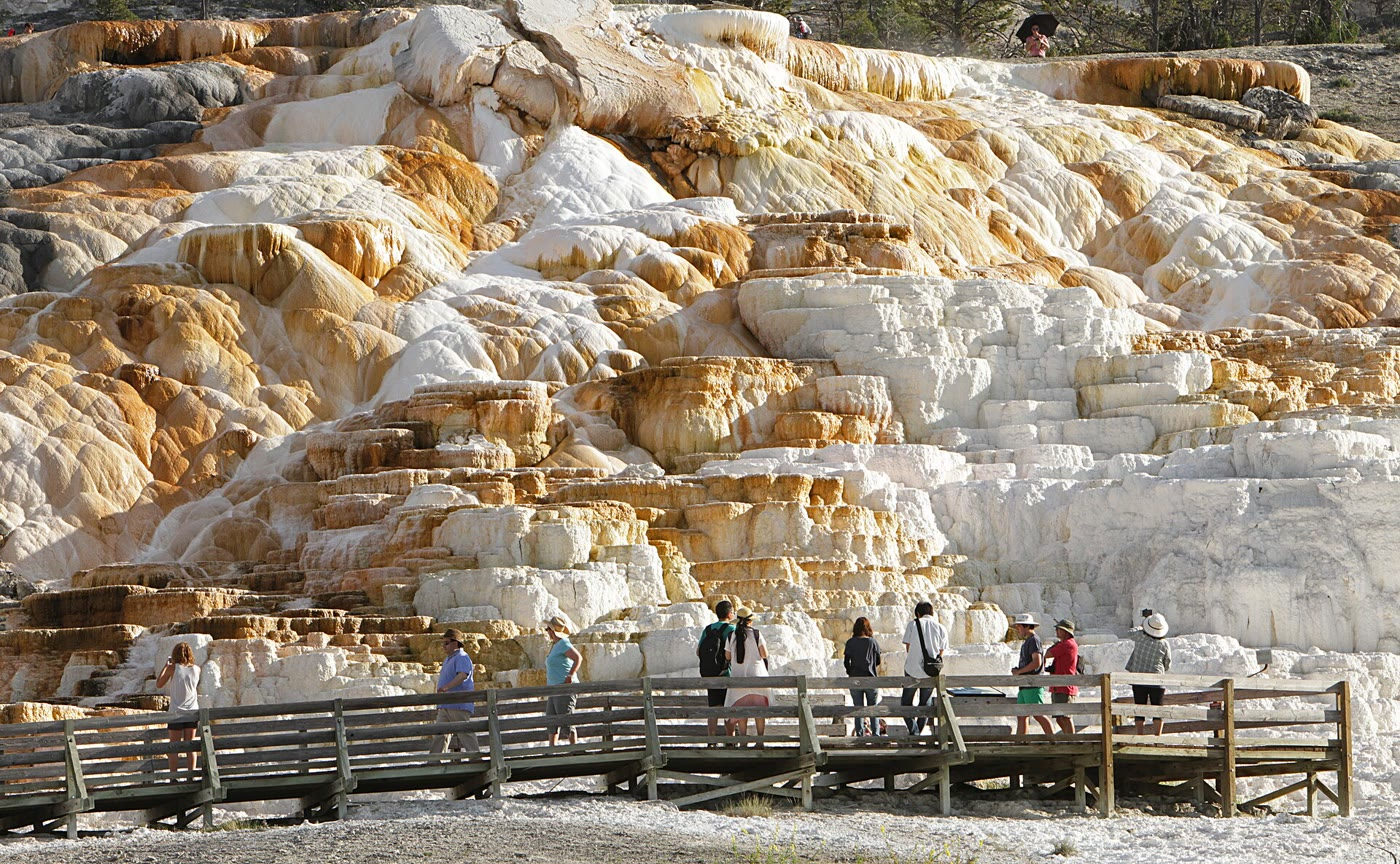
\includegraphics[width=\linewidth]{images/book5/b3-palette-spring-travertine.jpg}

{\scriptsize पैलेट स्प्रिंग की ट्रैवर्टीन वेदिकाएँ, मैमथ हॉट स्प्रिंग्स, जिनमें
पैमाने के लिए एक लकड़ी का पथ और आगंतुक दिख रहे हैं। NPS की फ़ोटो, Jim Peaco द्वारा, सार्वजनिक डोमेन।}
\end{minipage}
\end{inthefield}
% ledger: photo:b3-palette-spring, usgsyvo:travertine, nps:travertine-terraces

\section{सिलिकेट अपक्षय गतिकी}\label{sec:b3:water-rock-interaction:kinetics}

सिलिकेट कैल्साइट से कहीं अधिक धीरे विलयित होते हैं, और
जल शायद ही कभी उनके साथ साम्य तक पहुँचता है: उनके विलयन को एक दर से वर्णित करना पड़ता है।

\begin{definition}[खनिज विलयन दर नियम]\label{def:b3:water-rock-interaction:rate-law}
\emph{खनिज विलयन दर नियम}\index{खनिज विलयन दर नियम}
प्रति इकाई खनिज-पृष्ठ पर विलयन की दर
\unit{mol.m^{-2}.s^{-1}} में, अम्लीय, उदासीन और क्षारकीय क्रियाविधियों के योग के रूप में देता है,
\[
r = \sum_j k_j\,e^{-\frac{E_j}{R}\left(\frac1T - \frac1{298.15}\right)}\,
a_{\ce{H+}}^{n_j}\,\bigl(1 - \Omega^{p_j}\bigr)^{q_j},
\]
दर-स्थिरांक $k_j$ (\qty{25}{\celsius} पर), सक्रियण ऊर्जाएँ $E_j$,
अभिक्रिया कोटियाँ $n_j$ (क्षारकीय क्रियाविधि के लिए ऋणात्मक), और दो घातांक
$p_j$, $q_j$, जिन्हें प्रायः 1 माना जाता है।
\end{definition}
% ledger: pk04:rate-law

\begin{proposition}[साम्य से दूर और साम्य के निकट]\label{prop:b3:water-rock-interaction:affinity}
$p = q = 1$ हो तो दर जल की संतृप्ति पर निर्भर नहीं करती,
जब $\Omega \ll 1$ हो, और साम्य के निकट वह \omterm{def:b3:water-rock-interaction:si}{संतृप्ति सूचकांक} के
समानुपाती होती है: $r \approx -2.303\,r_\infty\,\mathrm{SI}$, जहाँ
$r_\infty$ साम्य से दूर की दर है।
\end{proposition}

\begin{proof}
गुणक $1 - \Omega = 1 - 10^{\mathrm{SI}}$ है। $\mathrm{SI} \ll 0$ के लिए यह
1 की ओर प्रवृत्त होता है; $\mathrm{SI}$ के 0 के निकट होने पर, $10^{\mathrm{SI}} \approx 1 +
2.303\,\mathrm{SI}$।
\end{proof}

दर-स्थिरांक ताज़े खनिज चूर्णों पर प्रयोगशाला प्रयोगों से आते हैं,
प्रवाह-रिएक्टरों में, जो साम्य से दूर रखे गए थे। नीचे की आकृति
चार खनिजों के लिए \qty{25}{\celsius} पर दर नियम दिखाती है। प्रत्येक वक्र V या
U जैसा होता है: प्रोटॉन अम्लीय जल में विलयन को तेज़ करते हैं, हाइड्रॉक्साइड क्षारकीय जल में, और
बीच में उदासीन क्रियाविधि एक निचली सीमा तय करती है। ओलिवीन pH 5 पर अल्बाइट से लगभग तीन
परिमाण-कोटियाँ तेज़ी से घुलता है। इसी कारण यह सामान्य सिलिकेटों में सबसे पहले
मृदा से लुप्त होने वाला खनिज है। अल्बाइट और फ़ॉर्स्टेराइट की सक्रियण ऊर्जाएँ
65 से \qty{79}{kJ/mol} के बीच हैं, जिसके कारण उनकी दरें
\qty{25}{\celsius} पर \qty{10}{\celsius} की तुलना में चार से पाँच गुना तेज़ होती हैं।
% ledger: pk04:rates

क्षेत्र की दरें परिमाण की कोटियों तक कम होती हैं। स्तंभ-प्रयोगों में एक
ताज़े पिसे ग्रेनाइट पर प्लैजियोक्लेज़ की दर छह वर्षों में लगातार गिरकर
\qty{7.0e-14}{mol.m^{-2}.s^{-1}} रह गई; वही ग्रेनाइट, जो प्राकृतिक रूप से अपक्षयित होकर आंशिक रूप से
कैओलिनाइट में बदल चुका था, उन्हीं परिस्थितियों में \qty{2.1e-15}{mol.m^{-2}.s^{-1}} पर घुला,
और दोनों अब भी उस दर से कहीं अधिक तेज़ हैं
जो अपक्षय-परिच्छेदिका में स्वयं मापी गई। अनेक खनिजों और आयुओं पर
दर, खनिज के अपक्षयित होने के समय $t$ के साथ, इस प्रकार घटती है: $R =
\num{3.1e-13}\,t^{-0.61}$ (mol\,m$^{-2}$\,s$^{-1}$, $t$ वर्षों में)। इस गिरावट का एक भाग
खनिज में है, जिसकी सबसे अभिक्रियाशील सतहें पहले घुल जाती हैं;
शेष परिवेश में है: धीमा जल, थोड़े तरल के लिए बहुत खनिज, और
रंध्र-जल साम्य के निकट, जहाँ ऊपर की प्रतिज्ञप्ति के अनुसार दर
छोटी हो जाती है।
% ledger: whitebrantley03:rates

\begin{omfigure}
\begin{tikzpicture}
\begin{axis}[omrecord, width=0.74\linewidth, height=0.46\linewidth,
  xlabel={pH}, ylabel={$\log r$ (\unit{mol.m^{-2}.s^{-1}})},
  xmin=0, xmax=14, ymin=-14.5, ymax=-6, clip=false,
  xtick={0,2,4,6,8,10,12,14}, ytick={-14,-12,-10,-8,-6},
  yticklabels={$-14$,$-12$,$-10$,$-8$,$-6$},
  tick label style={font=\scriptsize}, label style={font=\small},
  legend style={font=\scriptsize, legend cell align=left, at={(1.03,0.5)}, anchor=west}]
% computed in figdata/bachelor-3/weathering_rates.py
\addplot[green!45!black, thick] table[x=ph, y=forsterite] {figdata/out/bachelor-3-weathering_rates-curves.dat};
\addlegendentry{फ़ॉर्स्टेराइट}
\addplot[omDef, thick] table[x=ph, y=albite] {figdata/out/bachelor-3-weathering_rates-curves.dat};
\addlegendentry{अल्बाइट}
\addplot[red!70!black, thick, densely dashed] table[x=ph, y=kfeldspar] {figdata/out/bachelor-3-weathering_rates-curves.dat};
\addlegendentry{K-फ़ेल्सपार}
\addplot[black, thick, densely dotted] table[x=ph, y=kaolinite] {figdata/out/bachelor-3-weathering_rates-curves.dat};
\addlegendentry{कैओलिनाइट}
\end{axis}
\end{tikzpicture}

\par\smallskip{\small साम्य से दूर की विलयन दरें
\qty{25}{\celsius} पर, pH के सापेक्ष, एक प्रकाशित संकलन से लिए गए
प्रयोगशाला दर-प्राचल। ओलिवीन का अंत्य-सदस्य फ़ॉर्स्टेराइट
संकलन में कोई क्षारकीय क्रियाविधि नहीं रखता; इसका वक्र उदासीन निचली सीमा पर गिरना बंद कर देता है।}\label{fig:b3:water-rock-interaction:rates}
\end{omfigure}
% ledger: pk04:rates

\begin{definition}[अपक्षय की अवस्थाएँ]\label{def:b3:water-rock-interaction:regimes}
किसी भूदृश्य में रासायनिक अपक्षय \emph{आपूर्ति-सीमित अवस्था}\index{आपूर्ति-सीमित अवस्था} में होता है, जब वह
उस दर से सीमित हो, जिस दर से अपरदन ताज़ा खनिजों को
अपक्षय-मोर्चे तक लाता है, और
\emph{अपक्षय-सीमित अवस्था}\index{अपक्षय-सीमित अवस्था} में होता है, जब ताज़ा खनिज प्रचुर हों
और अभिक्रियाओं की दर उसे सीमित करे।
\end{definition}

छोटे जलग्रहण क्षेत्रों के एक संकलन में दोनों दिखते हैं। जहाँ अपरदन धीमा है, मोटी और निक्षालित मिट्टी के नीचे, मंद उच्चावच पर,
अपक्षय-फ़्लक्स अपरदन-दर का अनुसरण करता है; जो भी ताज़ा चट्टान पहुँचती है, वह पूरी तरह निक्षालित हो जाती है,
और गर्म या नम जलवायु से बहुत कम बदलाव आता है। जहाँ अपरदन तेज़ है, खड़े पर्वतों में,
अपक्षय-फ़्लक्स अपवाह के साथ बढ़ता है, अपरदन-दर के वर्गमूल के रूप में,
और तापमान के साथ, जिसकी स्पष्ट सक्रियण ऊर्जा $74 \pm
\qty{29}{kJ/mol}$ है। केवल दूसरी अवस्था में ही सिलिकेट-अपक्षय
तापस्थापी के रूप में कार्य कर सकता है,
जैसा पुस्तक 4 (स्नातक वर्ष 2) में वर्णित है।
% ledger: west05:regimes

कौन-सा द्वितीयक खनिज अपक्षय-जल बनाता है, यह
एक अन्य आरेख पर पढ़ा जाता है।

\begin{definition}[सक्रियता आरेख]\label{def:b3:water-rock-interaction:activity-diagram}
\emph{सक्रियता आरेख (खनिज स्थायित्व)}\index{सक्रियता आरेख (खनिज स्थायित्व)}
किसी जल के सक्रियता-अनुपातों के एक तल को, जैसे
$\log(a_{\ce{K+}}/a_{\ce{H+}})$ बनाम $\log a_{\ce{H4SiO4}}$ पर, उन क्षेत्रों में बाँटता है
जिनमें रासायनिक तंत्र का प्रत्येक खनिज स्थायी होता है।
\end{definition}

\begin{proposition}[सक्रियता आरेख की सीमाएँ]\label{prop:b3:water-rock-interaction:boundaries}
तंत्र \ce{K2O}--\ce{Al2O3}--\ce{SiO2}--\ce{H2O} में, जहाँ ठोसों में एल्यूमिनियम संरक्षित है
और जल की सक्रियता एक हो, तो एक खनिज जिसमें $k$ पोटैशियम, $a$ एल्यूमिनियम और
$s$ सिलिकन परमाणु प्रति सूत्र हों, और विलयन-स्थिरांक $K$ (\ce{K+},
\ce{Al^3+}, \ce{H4SiO4} में घुलने पर) निम्न संबंध निर्धारित करता है
\[
\log\frac{a_{\ce{Al^3+}}}{a_{\ce{H+}}^3} = \frac{\log K - kX - sY}{a},
\qquad X = \log\frac{a_{\ce{K+}}}{a_{\ce{H+}}},\quad Y = \log a_{\ce{H4SiO4}}.
\]
स्थायी खनिज सबसे निम्न एल्यूमिनियम सक्रियता देता है, और दो खनिजों के बीच की सीमा
$(Y, X)$ में एक सीधी रेखा होती है।
\end{proposition}

\begin{proof}
आवेश-संतुलन से विलयन $h = k + 3a$ प्रोटॉन उपभुक्त करता है, अतः $a\log
a_{\ce{Al^3+}} = \log K + h\log a_{\ce{H+}} - k\log a_{\ce{K+}} - s\log
a_{\ce{H4SiO4}}$; $a$ से भाग देने और $3\log a_{\ce{H+}}$ को बाईं ओर लाने पर
व्यंजक प्राप्त होता है। एक खनिज के साथ साम्य में स्थित जल
उन खनिजों के प्रति असंतृप्त होता है जिन्हें अधिक एल्यूमिनियम चाहिए, और
जिन्हें कम चाहिए उनके प्रति अतिसंतृप्त होता है, अतः सबसे कम विलेय खनिज
स्थायी होता है। $X$ और $Y$ में रैखिक, ऐसे दो व्यंजकों को बराबर करने पर एक रेखा प्राप्त होती है।
\end{proof}

\qty{25}{\celsius} पर स्थिरांकों के साथ, गिब्साइट
$\log a_{\ce{H4SiO4}} = -4.39$ (\qty{2.4}{mg/L} सिलिका) पर कैओलिनाइट को रास्ता देता है,
$\log(a_{\ce{K+}}/a_{\ce{H+}}) = 1.55$ पर कैओलिनाइट मस्कोवाइट को रास्ता देता है, और K-फ़ेल्सपार
केवल पोटैशियम और सिलिका से समृद्ध जल में स्थायी होता है। यह आरेख पुस्तक 3 (स्नातक वर्ष 1) के
अपक्षय-अनुक्रम को संख्याओं में प्रस्तुत करता है: तनु जल, जो पोटैशियम और सिलिका को बहा ले जाता है,
फ़ेल्सपार को गिब्साइट तक छील देता है; वह जल जो अधिक सिलिका रखता है,
कैओलिनाइट बनाता है; और वह जो गहराई की तरह अधिक पोटैशियम रखता है,
अभ्रक बनाता है।
% ledger: phreeqc:silicates

\begin{omfigure}
\begin{tikzpicture}
\begin{axis}[omrecord, width=0.66\linewidth, height=0.5\linewidth,
  xlabel={$\log a_{\ce{H4SiO4}}$}, ylabel={$\log(a_{\ce{K+}}/a_{\ce{H+}})$},
  xmin=-6, xmax=-2, ymin=0, ymax=10, clip=false,
  xtick={-6,-5,-4,-3,-2}, xticklabels={$-6$,$-5$,$-4$,$-3$,$-2$},
  tick label style={font=\scriptsize}, label style={font=\small}]
% computed in figdata/bachelor-3/activity_diagram.py
\addplot[black, thick, unbounded coords=jump] table[x=y, y=x] {figdata/out/bachelor-3-activity_diagram-lines.dat};
\addplot[omDef, densely dashed] table[x=y, y=x] {figdata/out/bachelor-3-activity_diagram-quartz.dat};
\addplot[omDef, densely dotted] table[x=y, y=x] {figdata/out/bachelor-3-activity_diagram-amorph.dat};
\addplot[red!70!black, only marks, mark=*, mark size=1.8pt] table[x=y, y=x] {figdata/out/bachelor-3-activity_diagram-samples.dat};
\node[font=\small] at (axis cs:-5.4,0.8) {गिब्साइट};
\node[font=\small] at (axis cs:-3.25,0.75) {कैओलिनाइट};
\node[font=\small] at (axis cs:-4.6,5.0) {मस्कोवाइट};
\node[font=\small] at (axis cs:-3.3,9.3) {K-फ़ेल्सपार};
\node[font=\scriptsize, omDef, anchor=south] at (axis cs:-3.98,10) {क्वार्ट्ज़};
\node[font=\scriptsize, omDef, anchor=south] at (axis cs:-2.71,10) {अनाकार सिलिका};
\node[font=\scriptsize, red!70!black, anchor=west] at (axis cs:-4.58,0.38) {A};
\node[font=\scriptsize, red!70!black, anchor=west] at (axis cs:-3.80,1.29) {B};
\node[font=\scriptsize, red!70!black, anchor=west] at (axis cs:-3.48,4.08) {C};
\end{axis}
\end{tikzpicture}

\par\smallskip{\small स्थायित्व क्षेत्र, तंत्र
\ce{K2O}--\ce{Al2O3}--\ce{SiO2}--\ce{H2O} में \qty{25}{\celsius} पर, क्वार्ट्ज़ की संतृप्ति
(धारीदार) और अनाकार सिलिका (बिंदीदार) के साथ। तीन काल्पनिक जल: A, एक तनु
उष्णकटिबंधीय धारा; B, ग्रेनाइट पर एक धारा; C, ग्रेनाइट में एक गहरा
भूजल।}\label{fig:b3:water-rock-interaction:activity}
\end{omfigure}
% ledger: phreeqc:silicates

\section{जलतापीय तरल}\label{sec:b3:water-rock-interaction:hydrothermal}

कटक या अंतर्वेधन के पास भूपर्पटी में परिसंचरण करता गर्म जल,
उसके पार जाने वाली चट्टान के साथ ऑक्सीजन का विनिमय करता है। उच्च तापमान पर
चट्टान और जल के बीच प्रभाजन छोटा होता है, और दोनों समस्थानिक साम्य की ओर बढ़ते हैं:
हल्का वर्षा-जल चट्टान को हल्का बनाता है, और
जल को भारी। चट्टान कितनी दूर खिसकी है, इससे मापा जाता है कि कितना जल
गुज़र चुका है।

\begin{definition}[जल--चट्टान अनुपात]\label{def:b3:water-rock-interaction:water-rock-ratio}
किसी जलतापीय तंत्र का \emph{जल--चट्टान अनुपात}\index{जल--चट्टान अनुपात} $W/R$ उस जल के
द्रव्यमान का, जो किसी चट्टान-द्रव्यमान के साथ विनिमय हुआ है,
उस चट्टान-द्रव्यमान से भाग देने पर प्राप्त होता है।
\end{definition}

\begin{proposition}[ऑक्सीजन समस्थानिकों से जल--चट्टान अनुपात]\label{prop:b3:water-rock-interaction:wr}
मान लीजिए $\delta_r^i$ आरंभिक मान वाली एक चट्टान, आरंभिक $\delta_w^i$ वाले जल के साथ
ऑक्सीजन का विनिमय करे, जब तक वह $\delta_r^f$ तक न पहुँचे, उस जल के साथ साम्य में
जिससे वह अंत में मिला था, $\Delta = \delta_r^f - \delta_w^f$, और $c_r$ तथा $c_w$ चट्टान और जल की
ऑक्सीजन सांद्रताएँ हों। बंद तंत्र (जल का एक बैच) में और खुले तंत्र
(जिसमें जल एक बार बहता है) में,
\[
\frac WR\Big|_{\text{बंद}} = \frac{c_r}{c_w}\,
\frac{\delta_r^f - \delta_r^i}{\delta_w^i - \delta_r^f + \Delta},
\qquad
\frac WR\Big|_{\text{खुला}} = \frac{c_r}{c_w}\,
\ln\!\left(\frac{\delta_r^f - \delta_r^i}{\delta_w^i - \delta_r^f + \Delta} + 1\right).
\]
\end{proposition}

\begin{proof}
बंद तंत्र: ऑक्सीजन-18 संरक्षित रहता है, $c_wW\delta_w^i + c_rR\delta_r^i = c_wW
\delta_w^f + c_rR\delta_r^f$, जहाँ $\delta_w^f = \delta_r^f - \Delta$ है;
इससे $W/R$ के लिए हल कीजिए। खुले तंत्र में एक भाग $\mathrm dW$ $\delta_w^i$ पर प्रवेश करता है और
चट्टान के साथ साम्य में, $\delta_r - \Delta$ पर बाहर निकलता है, अतः $c_rR\,\mathrm d\delta_r
= c_w(\delta_w^i - \delta_r + \Delta)\,\mathrm dW$। चर पृथक करने पर,
$\int_{\delta_r^i}^{\delta_r^f}\mathrm d\delta_r/(\delta_w^i - \delta_r +
\Delta) = (c_w/c_r)\,W/R$ प्राप्त होता है, और समाकल $-\ln[(\delta_w^i - \delta_r^f
+ \Delta)/(\delta_w^i - \delta_r^i + \Delta)]$ है, जो वही व्यंजक है।
\end{proof}

ऑक्सीजन के लिए $c_r/c_w$ लगभग 0.5 होता है। एक ही विस्थापन के लिए खुला तंत्र सदा
बंद तंत्र से कम जल माँगता है, क्योंकि हर भाग यथासंभव भारी होकर
बाहर निकलता है। कई अंतर्वेधनों के चारों ओर पार्श्व चट्टान का $\delta^{18}\mathrm O$
निम्न मानों का एक लक्ष्य-वृत्त जैसा क्षेत्र बनाता है, लगभग $+6$ से घटकर
0 से नीचे तक, जिसका केंद्र वहाँ होता है जहाँ सबसे अधिक जल गुज़रा था; जलतापीय
तरल के अयस्क प्रायः सबसे निचले समोच्च के भीतर मिलते हैं, जिससे यह मानचित्र अन्वेषण
का एक उपकरण बन जाता है।
% ledger: white13c9:water-rock

\begin{omfigure}
\begin{tikzpicture}[font=\small, >=Stealth]
\draw[thick, fill=black!6] (0,0) rectangle (4,2.2);
\node at (2,1.55) {चट्टान, द्रव्यमान $R$};
\node at (2,0.95) {$\delta_r^i \to \delta_r^f$};
\node[font=\scriptsize] at (2,0.4) {$T$ तापमान पर विनिमय};
\draw[->, thick, omDef] (-2.6,1.1) -- (-0.1,1.1);
\node[omDef, anchor=south, align=center, font=\scriptsize] at (-1.35,1.15) {जल अंदर\\ $\delta_w^i$, $\mathrm dW$};
\draw[->, thick, red!70!black] (4.1,1.1) -- (6.6,1.1);
\node[red!70!black, anchor=south, align=center, font=\scriptsize] at (5.35,1.15) {जल बाहर\\ $\delta_r - \Delta$};
\node[anchor=north, font=\scriptsize, align=center] at (2,-0.15) {खुला तंत्र: हर भाग एक बार बहता है और\\ अंतिम बार मिली चट्टान के साथ साम्य में निकलता है};
\end{tikzpicture}

\par\smallskip{\small जलतापीय प्रणाली का बॉक्स मॉडल। बंद तंत्र में
जल का एक बैच तब तक चट्टान के साथ रहता है जब तक दोनों साम्य में नहीं आ जाते;
खुले तंत्र में जल बहकर गुज़रता है, और हर भाग के साथ चट्टान
जल की ओर थोड़ा खिसकती है।}\label{fig:b3:water-rock-interaction:box}
\end{omfigure}

\begin{definition}[अभिक्रिया-पथ मॉडल]\label{def:b3:water-rock-interaction:reaction-path}
\emph{अभिक्रिया-पथ मॉडल}\index{अभिक्रिया-पथ मॉडल} किसी जल के संघटन और
उसके बनाए खनिजों को अभिक्रिया के आगे बढ़ने के साथ अनुसरण करता है,
अभिकारक की थोड़ी-थोड़ी मात्राएँ जोड़कर (कोई खनिज घुलना, कोई गैस निकलना,
ऊष्मा हटाना) और हर चरण पर स्पीशिएशन तथा \omterm{def:b3:water-rock-interaction:si}{संतृप्ति सूचकांक} पुनः परिकलित करके,
जो भी खनिज संतृप्ति तक पहुँचता है उसे अवक्षेपित करते हुए।
\end{definition}

\omterm{def:b3:water-rock-interaction:reaction-path}{अभिक्रिया-पथ मॉडल} को सप्ताहांत समस्या के सोते पर, चरण-दर-चरण गैस निकालते हुए, चलाने पर
जैसे ही कैल्साइट का सूचकांक शून्य से ऊपर जाता है, वह अवक्षेपित हो जाता है;
ग्रेनाइट और वर्षा-जल पर चलाने पर यह सबसे पहले गिब्साइट, फिर कैओलिनाइट, फिर
अभ्रक बनाता है, जब जल सिलिका और पोटैशियम एकत्र करता है, और सक्रियता आरेख पर एक पथ खींचता है।
स्पीशिएशन प्रोग्राम यह काम ऐसे साम्य स्थिरांकों के डेटाबेस के साथ करते हैं,
जैसे इस अध्याय में प्रयुक्त किए गए।
% ledger: phreeqc:silicates

\section{अभ्यास}

\begin{exercise}[$\star$]\label{exo:b3:water-rock-interaction:1}
एक जल में (\unit{mg/L} में) \ce{Ca} 48, \ce{Mg} 9.7, \ce{Na} 23, \ce{K} 3.9,
\ce{HCO3} 183, \ce{Cl} 35.5 और \ce{SO4} 48 है; इसकी आवेश-संतुलन
त्रुटि परिकलित कीजिए। क्या यह विश्लेषण स्वीकार्य है?
\end{exercise}

\begin{exercise}[$\star$]\label{exo:b3:water-rock-interaction:2}
आयनिक सामर्थ्य 0.0050 पर
\ce{Ca^2+}, \ce{HCO3-} और \ce{SO4^2-} के सक्रियता गुणांक परिकलित कीजिए।
\end{exercise}

\begin{exercise}[$\star$]\label{exo:b3:water-rock-interaction:3}
जिप्सम-युक्त मार्ल से बहता एक जल \qty{3.0}{mmol/L} कैल्शियम और
\qty{4.0}{mmol/L} सल्फ़ेट रखता है, आयनिक सामर्थ्य 0.016 पर। जिप्सम का
\omterm{def:b3:water-rock-interaction:si}{संतृप्ति सूचकांक} परिकलित कीजिए। क्या यह जल अब भी जिप्सम घोल सकता है?
\end{exercise}

\begin{exercise}[$\star$]\label{exo:b3:water-rock-interaction:4}
एक भू-जल में \qty{12}{mg/L} सिलिका है, जिसे \ce{SiO2} के रूप में दर्शाया गया है और
\ce{H4SiO4} के रूप में मौजूद है। क्वार्ट्ज़ और अनिराकार सिलिका के लिए
\qty{25}{\celsius} पर उसके \omterm{def:b3:water-rock-interaction:si}{संतृप्ति सूचकांक} परिकलित कीजिए।
\end{exercise}
% ledger: phreeqc:silicates

\begin{exercise}[$\star\star$]\label{exo:b3:water-rock-interaction:5}
सक्रियता गुणांकों को 1 मानते हुए, खुले तंत्र द्वारा घुलाए गए कैल्शियम को
$P_{\ce{CO2}} = 10^{-2}$~atm पर \qty{25}{\celsius} और
\qty{10}{\celsius} पर, \unit{mmol/L} और \unit{mg/L} में परिकलित कीजिए।
\end{exercise}

\begin{exercise}[$\star\star$]\label{exo:b3:water-rock-interaction:6}
\qty{25}{\celsius} पर एक जल का pH 7.60 है और उसमें
\qty{4.0}{mmol/L} बाइकार्बोनेट है। सक्रियता गुणांक 1 मानते हुए, उसकी घुली कार्बन
डाइऑक्साइड और कार्बोनेट, उसका $P_{\ce{CO2}}$ और
घुले अकार्बनिक कार्बन में प्रत्येक स्पीशीज़ का अंश परिकलित कीजिए।
\end{exercise}

\begin{exercise}[$\star\star$]\label{exo:b3:water-rock-interaction:7}
pH 5 वाले मृदा-जल में एक एल्बाइट कण \qty{1}{mm} व्यास का गोला है, जो
\qty{25}{\celsius} पर चित्र में दी गई दर से घुलता है, $\log r = -12.09$।
\qty{101.31}{cm^3/mol} के मोलर आयतन के साथ, इसकी त्रिज्या कितनी तेज़ी से
घटती है, और यह कितने समय तक टिकता है?
\end{exercise}
% ledger: pk04:rates, phreeqc:silicates

\begin{exercise}[$\star\star$]\label{exo:b3:water-rock-interaction:8}
एल्बाइट की उदासीन विलयन दर ($E =
\qty{69.8}{kJ/mol}$) \qty{5}{\celsius} से \qty{25}{\celsius} तक कितने गुना बढ़ती है? और
$E = \qty{74}{kJ/mol}$ वाले अपक्षय प्रवाह के लिए?
\end{exercise}
% ledger: pk04:rates, west05:regimes

\begin{exercise}[$\star\star$]\label{exo:b3:water-rock-interaction:9}
सक्रियता आरेख की कैओलिनाइट--मस्कोवाइट सीमा को स्थिरांकों
$\log K = 7.435$ (कैओलिनाइट, 2 Al, 2 Si) और $12.703$ (मस्कोवाइट, 1 K, 3 Al, 3 Si) से व्युत्पन्न कीजिए।
\qty{25}{\celsius} पर एक जल में \qty{2.0}{mg/L} पोटैशियम,
\qty{15}{mg/L} सिलिका और pH 7.0 है: वह कौन-सा खनिज बनाता है?
\end{exercise}
% ledger: phreeqc:silicates

\begin{exercise}[$\star\star\star$]\label{exo:b3:water-rock-interaction:10}
अंतर्वेधन के निकट $\delta^{18}\mathrm O = +6$ वाला एक ग्रैनोडायोराइट
$-2$ (\unit{\permil}) पर पाया जाता है। वायुमंडलीय जल का मान $-13$ था, और विनिमय के तापमान पर
चट्टान जल से \qty{2}{\permil} भारी थी।
$c_r/c_w = 0.5$ लेकर बंद तंत्र और
खुले तंत्र के लिए \omterm{def:b3:water-rock-interaction:water-rock-ratio}{जल--चट्टान अनुपात} परिकलित कीजिए, और समझाइए कि वे क्यों भिन्न हैं।
\end{exercise}
% ledger: white13c9:water-rock

\begin{exercise}[$\star\star\star$]\label{exo:b3:water-rock-interaction:11}
मृदा गैस से युक्त वर्षा-जल $P_{\ce{CO2}} = 10^{-1.5}$~atm दाब पर
\qty{10}{\celsius} पर एक चूना-पत्थर तक पहुँचता है। सक्रियता गुणांक 1 मानकर,
यदि वह मृदा गैस के लिए खुला रहे, और यदि पहले उससे अलग कर दिया जाए, तो वह कितना कैल्सियम घोलता है, परिकलित कीजिए।
बंद स्थिति में उसकी कार्बन डाइऑक्साइड का कौन-सा भाग शेष रहता है,
और उसका अंतिम $P_{\ce{CO2}}$ क्या है?
\end{exercise}

\begin{exercise}[$\star\star\star$]\label{exo:b3:water-rock-interaction:12}
साम्य के निकट की दरों संबंधी प्रतिज्ञप्ति का उपयोग करके बताइए कि कोई खनिज अपनी
साम्यावस्था-से-दूर दर का कौन-सा भाग $\mathrm{SI} =
-2$, $-1$ और $-0.1$ पर घुलता है? प्रयोगशाला में 6 वर्ष की अभिक्रिया के बाद मापी गई एक दर
अध्याय के घात नियम का पालन करती है: वह किस गुणक से गिर चुकी होगी
\num{10000} वर्ष के बाद? दोनों प्रभावों को मिलाकर समझाइए कि क्षेत्र-दरें
इतनी कम क्यों होती हैं।
\end{exercise}
% ledger: whitebrantley03:rates

\section{समस्या: वार्डन चूना-पत्थर के नीचे का सोता}

\begin{problem}[{सप्ताहांत समस्या --- विश्लेषण, कार्बन डाइऑक्साइड और
एक काल्पनिक चूना-पत्थर सोते की संतृप्ति, और एक ग्रेनाइट धारा}]
\label{pb:b3:water-rock-interaction:1}
वार्डन पहाड़ियों के जुरासिक चूना-पत्थर की तलहटी में एक सोता
\qty{10}{\celsius} तापमान और pH 7.20 पर निकलता है। इसका विश्लेषण (\unit{mg/L} में) इस प्रकार है: \ce{Ca}
112, \ce{Mg} 4.0, \ce{Na} 7.0, \ce{K} 1.2, \ce{HCO3} 340, \ce{Cl} 11,
\ce{SO4} 14, \ce{NO3} 9. \qty{10}{\celsius} पर: $\log K_{\mathrm{cal}} =
-8.35$, $\log K_1 = -6.46$, $\log K_2 = -10.49$, $\log K_H = -1.27$ हैं।
अध्याय का विस्तारित डेबाई--ह्यूकेल समीकरण लागू कीजिए, आयन-युग्मों की उपेक्षा कीजिए और
वायु का $\log P_{\ce{CO2}} = -3.37$ लीजिए।

\medskip\noindent\textbf{भाग I --- विश्लेषण।}
\begin{enumerate}
\item विश्लेषण को \unit{mmol/L} में बदलिए।
\item आवेश-संतुलन त्रुटि परिकलित कीजिए। क्या विश्लेषण स्वीकार्य है?
\item आयनिक सामर्थ्य परिकलित कीजिए।
\item \ce{Ca^2+}, \ce{HCO3-} और
  \ce{CO3^2-} के सक्रियता गुणांक परिकलित कीजिए।
\item क्या यहाँ विस्तारित डेबाई--ह्यूकेल समीकरण वैध है?
\end{enumerate}

\medskip\noindent\textbf{भाग II --- कार्बन डाइऑक्साइड।}
\begin{enumerate}[resume]
\item बाइकार्बोनेट की सक्रियता परिकलित कीजिए।
\item घुली हुई कार्बन डाइऑक्साइड की सक्रियता परिकलित कीजिए।
\item सोते का $P_{\ce{CO2}}$ परिकलित कीजिए। वायु की तुलना में वह कितने गुना है,
  और कार्बन डाइऑक्साइड कहाँ से आ सकती है?
\item कार्बोनेट की सांद्रता और घुले अकार्बनिक कार्बन में हर स्पीशीज़ का
  भाग परिकलित कीजिए।
\item जाँचिए कि क्षारीयता लगभग पूर्णतः बाइकार्बोनेट है।
\end{enumerate}

\medskip\noindent\textbf{भाग III --- संतृप्ति और ट्रैवर्टीन।}
\begin{enumerate}[resume]
\item कैल्साइट का आयन सक्रियता गुणनफल और \omterm{def:b3:water-rock-interaction:si}{संतृप्ति सूचकांक}
  निकास पर परिकलित कीजिए।
\item क्या सोता कैल्साइट के साथ साम्यावस्था में है? क्या वह नलिका-सोता है या
  एक धीमा, विसरित सोता?
\item कैल्साइट के साथ साम्यावस्था में एक खुले तंत्र का कैल्सियम, सोते के
  $P_{\ce{CO2}}$ पर, प्रश्न 4 के सक्रियता गुणांकों के साथ परिकलित कीजिए,
  और विश्लेषण से तुलना कीजिए।
\item कैल्साइट बनने से पहले जल वायु में अपनी गैसें छोड़ता है। बाइकार्बोनेट की सक्रियता
  अपरिवर्तित रखते हुए उसका pH और \omterm{def:b3:water-rock-interaction:si}{संतृप्ति सूचकांक} परिकलित कीजिए।
\item कैल्साइट का अवक्षेपण करके वायु के साथ पुनः साम्यावस्था तक पहुँचने पर वह कितना कैल्सियम
  बनाए रखता है, इसका अनुमान लगाइए (खुला तंत्र, नई आयनिक सामर्थ्य पर सक्रियता गुणांक
  $3m$ पर), और प्रति लीटर कैल्साइट का द्रव्यमान।
\item सोता \qty{2.0}{L/s} की दर से बहता है और अपना निक्षेप
  \qty{400}{m^2} क्षेत्र पर फैलाता है। यदि सारा कैल्साइट वहीं रहे, तो
  \qty{2.71}{g/cm^3} घनत्व पर निक्षेप कितनी तेज़ी से बढ़ेगा?
\end{enumerate}

\medskip\noindent\textbf{भाग IV --- ग्रेनाइट धारा।} वार्डन ग्रेनाइट पर बहने वाली एक धारा,
मंद ढलानों पर मोटी मृदा के नीचे, (
\qty{25}{\celsius} पर) \qty{1.2}{mg/L} पोटैशियम, \qty{9.0}{mg/L} सिलिका और
pH 5.8 है।
\begin{enumerate}[resume]
\item सक्रियता आरेख पर इसकी स्थिति परिकलित कीजिए।
\item यह कौन-सा खनिज बनाती है? क्वार्ट्ज़ के लिए इसका \omterm{def:b3:water-rock-interaction:si}{संतृप्ति सूचकांक} परिकलित कीजिए।
\item किस सिलिका सांद्रता से नीचे यह गिब्साइट बनाएगी?
\item किस pH पर यह कैओलिनाइट--मस्कोवाइट सीमा तक पहुँचेगी?
\item इस जल में K-फ़ेल्सपार की साम्यावस्था से दूर की विलयन दर
  प्राचलों $\log k = -10.06$, $n = 0.500$ (अम्लीय);
  $-12.41$ (उदासीन); $-21.20$, $n = -0.823$ (क्षारीय) से परिकलित कीजिए।
\item क्या इस जलग्रहण क्षेत्र का अपक्षय अधिक संभावित रूप से आपूर्ति-सीमित है या
  अपक्षय-सीमित? क्यों?
\item \qty{74}{kJ/mol} की स्पष्ट सक्रियण ऊर्जा लेकर, किस गुणक से
  अपक्षय-सीमित फ़्लक्स \qty{10}{\celsius} और
  \qty{25}{\celsius} के बीच बदलेगा?
\item सोते के जल का उसके निकास पर कैल्साइट का \omterm{def:b3:water-rock-interaction:si}{संतृप्ति सूचकांक}
  बताइए।
\end{enumerate}
\end{problem}
% ledger: phreeqc:carbonate, phreeqc:silicates, hem85:debye-huckel, hem85:charge-balance, hem85:si, hem85:pco2, pk04:rates, west05:regimes, data:co2-mlo
